%% Copyright 2005 G. W. Knor
%%This work may be distributed and/or modified under the
% conditions of the LaTeX Project Public License, either version 1.3
% of this license or (at your option) any later version.
% The latest version of this license is in
% http://www.latex-project.org/lppl.txt
% and version 1.3 or later is part of all distributions of LaTeX
% version 2005/12/01 or later.
%%This work has the LPPL maintenance status "maintained".
%%The Current Maintainer of this work is G. W. Knor.
 
\documentclass{beamer}
\usepackage{graphicx}
\usepackage{sidecap}
\usepackage{courier}
\usepackage{listings}
\usepackage{hyperref}
\usepackage[utf8]
{inputenc}
\lstset{
    breaklines=true,
    breakatwhitespace=true,
    postbreak=\raisebox{0ex}[0ex][0ex]{\ensuremath{\color{red}\hookrightarrow\space}}
}
\setcounter{tocdepth}{1}

\definecolor{keywords}{RGB}{255,0,90}
\definecolor{comments}{RGB}{0,0,113}
\definecolor{red}{RGB}{160,0,0}
\definecolor{green}{RGB}{0,150,0}
 
\lstset{language=Python, 
        basicstyle=\ttfamily\small, 
        keywordstyle=\color{keywords},
        commentstyle=\color{comments},
        stringstyle=\color{red},
        showstringspaces=false,
        identifierstyle=\color{green},
        procnamekeys={def,class}}


\title{HowTo re}
\author{Dariusz Śmigiel}
\date{PyCon PL 2015}
\usetheme{Madrid}
\usecolortheme{seahorse}

\begin{document}

\begin{frame}
\titlepage
\end{frame}

\section*{Outline}
\begin{frame}
\tableofcontents
\end{frame}

\section{Section}
\subsection{Subsection}
\begin{frame}
\end{frame}

\section{History}
\subsection{Origins}
\begin{frame}
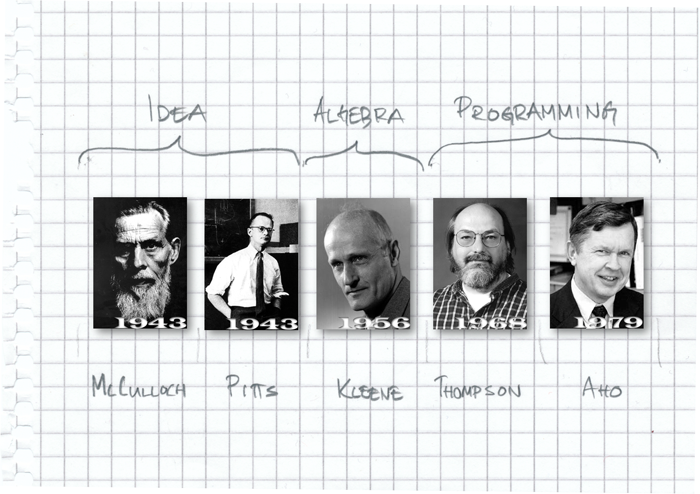
\includegraphics[width=1\textwidth]{images/history.png}
Staffan Noteberg: http://blog.staffannoteberg.com/
\end{frame}

\subsection{Python module}
\subsubsection{re module}
\begin{frame}
Delivering Quality and Value since Python 1.5 (December 31, 1997)
\pause
\subsubsection{regex module}
\item Deprecated old module `regex`, based on Perl-style patterns.
\item finally removed in Python 2.5.
\end{frame}

\section{Do I need it?}
\subsection{Matching}
\begin{frame}
\item "Does this string match the pattern?"
\item "Is there a match for the pattern anywhere in this string?"

\subsection{Modifying}
\item Replace part of it
\item Split into pieces
\end{frame}

\section{Under the hood}
\subsection{Implementation}
\begin{frame}
re patterns are compiled into bytecode
\pause
executed by engine written in C
\end{frame}

\subsection{Features}
\begin{frame}
re language is relatively small and restricted
\item not all possible string processing tasks can be done
\item some of them can be done, but expression would be very complicated
\end{frame}

\section{Simple patterns}
\subsection{Matching Characters}
\begin{frame}
(metacharacters)
. ^ $ * + ? { } [ ] \ | ( )
\end{frame}

\subsubsection{Class}
\begin{frame}
[ ]
Specifying a character class, which is set of characters that you wish to match
\item can be listed individually [abc]
\item can be given as range of characters, separated by '-' [a-c]
\end{frame}
\pause
Metacharacters are not active inside class
[akm$] will match any of: "a", "k", "m", "$"

\subsubsection{Complementing set}
\begin{frame}
[^5]
Including '^' as first character of the class: [^5] will match any except '5'
\end{frame}

\subsubsection{Backslash}
\begin{frame}
* escape metacharacters
For matching "[" or "\" you can use "\[" or "\\"
\end{frame}

\begin{frame}
* express predefined sets of characters: set of digits, letters, everything but whitespace
\item \d - any decimal digit, equivalent of [0-9]
\item \D - everything but decimal digit, equivalent of [^0-9]
\item \w - any alphanumeric: [a-zA-Z0-9_]
\item \W - any non-alpahnumeric: [^a-zA-Z0-9_]
\item \s - any whitespace character: [ \t\n\r\f\v] (space, tab, newline, return, ..., ...)
\item \S - any non-whitespace character: [^ \t\n\r\f\v]

\item \t -- tab character (ASCII 0x09),
\item \r -- carriage return (0x0D),
\item \n -- line feed (0x0A),
\item \a (bell, 0x07),
\item \e (escape, 0x1B),
\item \f (form feed, 0x0C),
\item \v (vertical tab, 0x0B)
NOTE! Remember that Windows text files use \r\n to terminate lines, while UNIX text files use \n.
\end{frame}

\subsubsection{Dot - '.'}
\begin{frame}
By default, matches anything except newline character.
There is alternate mode (re.DOTALL) where it matches everything. Used when it's needed to match "any character"
\end{frame}

\subsection{Repeating Things}
\subsubsection{Star -- "*"}
\begin{frame}
Doesn't match a character. Specifies that previous character can be matched zero or more times.
(ca*t) --> "ct", "cat", "caaat"
NOTE! RE engine has limitations steeming from the size of C's "int" type that will prevent it from matching over 2 billion "a" characters (2GB).
\end{frame}

\begin{frame}
* is greedy -- will try to repeat it as many times as possible

a[bcd]*b
Matches "a", zero or more letters from "bcd", and ends with "b"
"abcbd"
1. Matched "a"
2. Tries to match "abcbd" because of [bcd]* to the end of the string
3. Fails because current position is the end of the string, so cannot match "b"
4. "abcb" -- matches one less character
5. Fails, tries again "b" but current position is "d"
6. "abc", so [bcd]* matches only "bc"
7. "abcb", tries last character "b", and it's on current position
8. Success
\end{frame}

\subsubsection{Plus -- "+"}
\begin{frame}
Similar to "*", but requires at least one occurence of character
(ca+t) --> "cat", "caaat" but not "ct"
\end{frame}

\subsubsection{Quotation mark -- "?"}
\begin{frame}
Matches either once or zero times
"home-?brew" --> "homebrew", "home-brew"
\end{frame}

\subsubsection{"{m,n}"}
\begin{frame}
"m" and "n" are decimal numbers. There must be at least m repetitions, and at most n.
a/{1,3}b --> a/b, a//b, a///b
\pause
m and n can be ommited. When m ommited, there is zero, when n ommited, upper bound infinity (more precisely, 2 billions)
\end{frame}

\subsubsection{Equivalents}
\begin{frame}
{0,} == "*"
{1,} == "+"
{,1} == {0,1} == "?"
\end{frame}

REGULAR EXPRESSIONS

1. Compiling
REs are handled as strings because regular expressions aren’t part of the core Python language, and no special syntax was created for expressing them. (There are applications that don’t need REs at all, so there’s no need to bloat the language specification by including them.) Instead, the re module is simply a C extension module included with Python, just like the socket or zlib modules.

Backslash Plague

Characters	Stage
\section	Text string to be matched
\\section	Escaped backslash for re.compile()
"\\\\section"	Escaped backslashes for a string literal

to match a literal backslash, one has to write '\\\\' as the RE string, because the regular expression must be \\, and each backslash must be expressed as \\ inside a regular Python string literal.

Solution
Regular String	Raw string
"ab*"	r"ab*"
"\\\\section"	r"\\section"
"\\w+\\s+\\1"	r"\w+\s+\1"

\section{Bibliography}
\begin{frame}
Regular Expression HOWTO: https://docs.python.org/2/howto/regex.html
Python Docs: Library re: https://docs.python.org/2/library/re.html
Google for Education. Python Regular Expressions: https://developers.google.com/edu/python/regular-expressions?hl=en
Non-printable Characters: http://www.regular-expressions.info/nonprint.html
Core Python Applications programming: Regular expressions: http://www.informit.com/articles/article.aspx?p=1707750&seqNum=2
\end{frame}
\end{document}
